% CVPR 2022 Paper Template
% based on the CVPR template provided by Ming-Ming Cheng (https://github.com/MCG-NKU/CVPR_Template)
% modified and extended by Stefan Roth (stefan.roth@NOSPAMtu-darmstadt.de)

\documentclass[10pt,twocolumn,letterpaper]{article}

%%%%%%%%% PAPER TYPE  - PLEASE UPDATE FOR FINAL VERSION
% \usepackage[review]{cvpr}      % To produce the REVIEW version
% \usepackage{cvpr}              % To produce the CAMERA-READY version
\usepackage[pagenumbers]{cvpr} % To force page numbers, e.g. for an arXiv version

% Include other packages here, before hyperref.
\usepackage{subcaption}
\usepackage{graphicx}
\usepackage{amsmath}
\usepackage{amssymb}
\usepackage{booktabs}
\usepackage{array}
\usepackage{listings}
\usepackage{xcolor}
\lstset{
    basicstyle=\ttfamily\small,
    frame=single,
    breaklines=true,
    breakatwhitespace=true,
    columns=fullflexible,
    backgroundcolor=\color{gray!10},
    linewidth=\linewidth
}

% It is strongly recommended to use hyperref, especially for the review version.
% hyperref with option pagebackref eases the reviewers' job.
% Please disable hyperref *only* if you encounter grave issues, e.g. with the
% file validation for the camera-ready version.
%
% If you comment hyperref and then uncomment it, you should delete
% ReviewTempalte.aux before re-running LaTeX.
% (Or just hit 'q' on the first LaTeX run, let it finish, and you
%  should be clear).
\usepackage[pagebackref,breaklinks,colorlinks]{hyperref}


% Support for easy cross-referencing
\usepackage[capitalize]{cleveref}
\crefname{section}{Sec.}{Secs.}
\Crefname{section}{Section}{Sections}
\Crefname{table}{Table}{Tables}
\crefname{table}{Tab.}{Tabs.}

\begin{document}

%%%%%%%%% TITLE - PLEASE UPDATE
\title{\LARGE AI-Capstone: Project2 Report}
\author{I-Ting Chu, 111550093}
\maketitle

%%%%%%%%% BODY TEXT
\section{Introduction}
\label{sec:intro}

In this project, we aim to explore and compare the performance of different reinforcement learning (RL) algorithms across a variety of environments provided by OpenAI Gym. Specifically, I focus on three representative environments of increasing complexity: \textit{Classic/Pendulum-v1}, \textit{Box2D/LunarLander-v3}, and \textit{Atari/Pong-v5}. To address these tasks, we evaluate three widely used RL algorithms: PPO, DQN, and A2C. Our goal is to understand the strengths and limitations of each algorithm in different settings, as well as to investigate how various hyperparameters and implementation choices affect their learning behavior and convergence properties.

The following links show the trained agents performing in their respective environments:

\begin{itemize}
  \item \textbf{Pendulum-v1 (PPO)}: \href{https://youtube.com/shorts/AXvGvR7J8uM?feature=share}{link}
  \item \textbf{LunarLander-v3 (PPO)}: \href{https://youtu.be/Gy7jJm2cdyU}{link}
  \item \textbf{Pong-v5 (DQN)}: \href{https://youtube.com/shorts/BkrJ5J7AKvU?feature=share}{link}
\end{itemize}

%------------------------------------------------------------------------
\section{Methods}
\label{sec:methods}
In this section, we provide a brief overview of the three reinforcement learning algorithms applied in our experiments: Proximal Policy Optimization (PPO), Deep Q-Network (DQN), and Advantage Actor-Critic (A2C). Each of these methods represents a different class of RL algorithms and offers unique mechanisms for policy optimization.
\subsection{PPO}
Proximal Policy Optimization (PPO) is a policy gradient method that optimizes a clipped surrogate objective to prevent large policy updates and ensure training stability. The clipped objective is defined as:
\begin{equation*}
L^{\text{CLIP}}(\theta) = \hat{\mathbb{E}}_t \left[ \min\left( r_t(\theta) \hat{A}_t, \text{clip}(r_t(\theta), 1 - \epsilon, 1 + \epsilon) \hat{A}_t \right) \right]
\end{equation*}

where \( r_t(\theta) = \frac{\pi_\theta(a_t|s_t)}{\pi_{\theta_{\text{old}}}(a_t|s_t)} \) is the probability ratio between the new and old policies, and \( \hat{A}_t \) is the estimated advantage. The clipping parameter \( \epsilon \) (commonly 0.1 or 0.2) limits the change in policy to improve stability.~\cite{ppo}

\subsection{DQN}

Deep Q-Network (DQN) is a value-based method that learns to approximate the optimal Q-value function \( Q^*(s, a) \) using a neural network. The loss function for DQN is the mean squared error between the predicted and target Q-values:

\begin{equation*}
L(\theta) = \mathbb{E}_{(s,a,r,s')} \left[ \left( r + \gamma \max_{a'} Q_{\theta^{-}}(s', a') - Q_\theta(s, a) \right)^2 \right]
\end{equation*}

Here, \( Q_{\theta^{-}} \) is the target network, which is periodically updated to the current network \( Q_\theta \), and \( \gamma \) is the discount factor. Experience replay and target networks help stabilize training.~\cite{dqn}

\subsection{A2C}

Advantage Actor-Critic (A2C) is an on-policy algorithm that combines value-based and policy-based learning. It uses the advantage function \( \hat{A}_t = R_t - V(s_t) \) to reduce variance in policy updates. The actor and critic networks are updated with the following losses:

\textbf{Actor loss} (policy gradient):
\begin{equation*}
L^{\text{actor}} = -\log \pi_\theta(a_t|s_t) \cdot \hat{A}_t
\end{equation*}

\textbf{Critic loss} (value regression):
\begin{equation*}
L^{\text{critic}} = \left( R_t - V_\phi(s_t) \right)^2
\end{equation*}

The total loss is often the weighted sum:
\begin{equation*}
L = L^{\text{actor}} + c_1 L^{\text{critic}} - c_2 \mathcal{H}(\pi_\theta)
\end{equation*}

where \( \mathcal{H}(\pi_\theta) \) is an entropy bonus that encourages exploration, and \( c_1, c_2 \) are weighting coefficients.~\cite{a3c}

%------------------------------------------------------------------------
\section{Implementation Detail}
\label{sec:implementation}

In this section, we describe the implementation details of our experiments, including the framework we used and the environments selected for testing. All experiments were implemented in Python using the Stable-Baselines3 (SB3) library.

\subsection{Stable-Baselines3 (SB3)}
We use Stable-Baselines3 (SB3) \cite{sb3} version 2.6 as our main reinforcement learning framework. SB3 provides reliable and well-tested implementations of many modern RL algorithms, including PPO, DQN, and A2C. It offers a clean API for training and evaluation, as well as integration with Gymnasium environments and vectorized environments for efficient simulation.

\subsection{Testing Environments}
To evaluate the performance of each RL algorithm, we selected three diverse environments from different categories in OpenAI Gymnasium. The summary of their key properties is shown in Table~\ref{tab:env_comparison}. Also, the screenshots of each environment are shown in Figure~\ref{fig:env_images},~\ref{fig:pong}.

\begin{table}
  \centering
  \begin{tabular}{@{}l>{\raggedright\arraybackslash}p{5.5cm}@{}}
    \toprule
    Environment & Characteristics \\
    \midrule
    Pendulum-v1 & 3D state, continuous action, dense reward, 200 steps \\
    LunarLander-v3 & 8D state, discrete action (4), dense reward, 1000 steps \\
    Pong-v5 & $210 \times 160 \times 3$ image, discrete action (6), sparse reward, 10000 frames \\
    \bottomrule
  \end{tabular}
  \caption{Environment summary: state/action space, reward type, and episode length.}
  \label{tab:env_comparison}
\end{table}

\vspace{-0.5cm}
\begin{figure}[htbp]
  \centering
  
\includegraphics[width=0.45\linewidth]{assets/pendulum.png}
  \hfill
  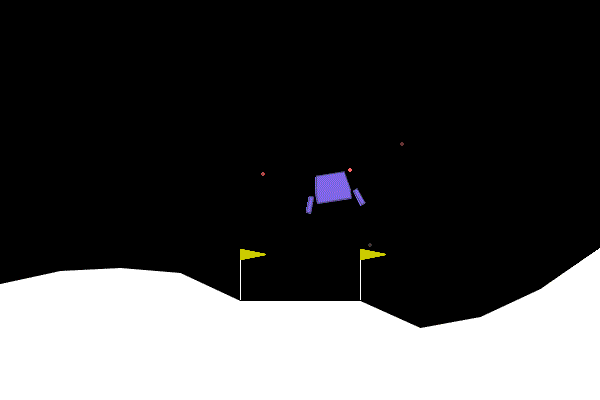
\includegraphics[width=0.45\linewidth]{assets/lunar_lander.png}
  \caption{Screenshots of Pendulum-v1, LunarLander-v3.}
  \label{fig:env_images}
\end{figure}

\subsubsection{Classic Control: Pendulum-v1}
Pendulum-v1 is a continuous control task where the goal is to keep a frictionless pendulum upright by applying torque. The task features a low-dimensional, continuous state space and a continuous action space. The reward is shaped and dense, penalizing angle deviation and control effort.

\subsubsection{Box2D: LunarLander-v3}
LunarLander-v3 is a physics-based 2D landing task. The agent must control a lander to safely land on a pad with discrete actions. The environment provides shaped rewards for progress and penalties for crashing or using excessive fuel.

\subsubsection{Atari: Pong-v5}
Pong-v5 is a classic Atari 2600 game and a standard benchmark for discrete, pixel-based deep RL. The agent observes raw pixel images and learns to control the paddle to defeat the opponent. Rewards are sparse and given only when a point is scored.
\begin{figure}[h]
    \centering
    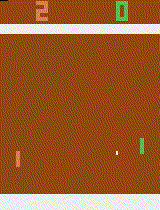
\includegraphics[width=0.4\linewidth]{assets/pong.png}
    \caption{Screenshots of Pong-v5.} 
    \label{fig:pong}
\end{figure}

\subsection{Metrics}
To evaluate training performance, we used \texttt{EvalCallback} provided by Stable-Baselines3~\cite{sb3}. During training, the model was periodically evaluated on a separate environment, and the best-performing model was saved. The evaluation setup is as follows:

\begin{lstlisting}
eval_callback = EvalCallback(
    eval_env,
    eval_freq=5000,
    deterministic=True,
    render=False,
)
\end{lstlisting}


We also monitored training progress using TensorBoard, focusing on:
\begin{itemize}
    \item \textbf{Loss curves} of the policy and value networks.
    \item \textbf{Episode rewards} over time to assess convergence speed and stability.
\end{itemize}

\subsection{Hyperparameters}
For fair comparisons across different algorithms and environments, we adopted the following default hyperparameter settings unless otherwise stated:

\begin{itemize}
    \item \textbf{Random seed}: 42
    \item \textbf{Learning rate}: $3 \times 10^{-4}$ 
    \item \textbf{Optimizer}: Adam 
    \item \textbf{Policy type}:
    \begin{itemize}
        \item \texttt{CnnPolicy} for Pong-v5 (trained on \texttt{cuda})
        \item \texttt{MlpPolicy} for Pendulum-v1 and LunarLander-v3 (trained on \texttt{cpu})
    \end{itemize}
    \item \textbf{gamma}: 0.99
    \item \textbf{Total timesteps}: 2,000,000
    \item \textbf{Evaluation frequency}: 5,000 steps
\end{itemize}

%------------------------------------------------------------------------
\section{Experiment}
\label{sec:experiment}

\subsection{Environments}
To compare convergence speed across environments, we trained PPO with the same setting (batch size = 128, total steps = 2,000,000) on Pendulum-v1, LunarLander-v3, and Pong-v5. The results are shown in Figure~\ref{fig:ppo_convergence}.

\begin{figure}[h]
  \centering
  \begin{subfigure}{0.9\linewidth}
    \centering
    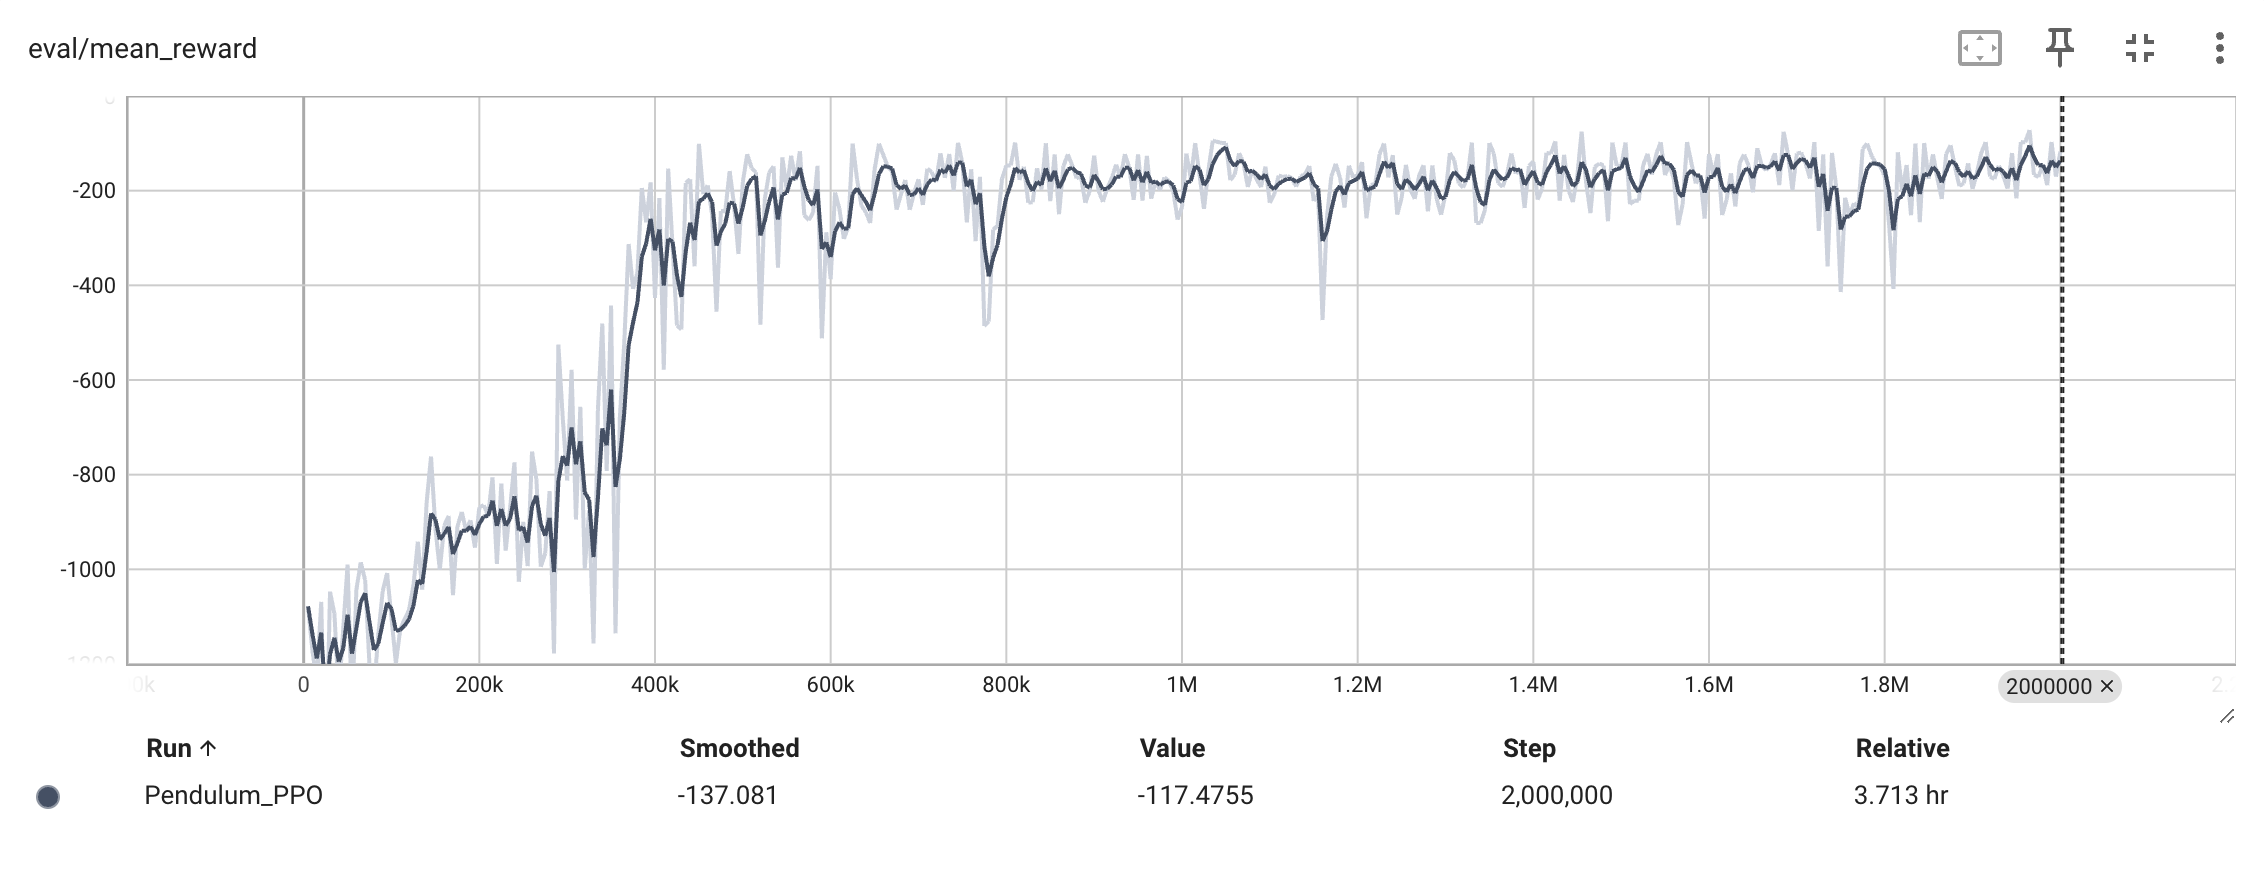
\includegraphics[width=\linewidth]{assets/4.1/Pendulum_PPO.png}
    \caption{Pendulum-v1}
  \end{subfigure}
  \vskip 0.5em
  \begin{subfigure}{0.9\linewidth}
    \centering
    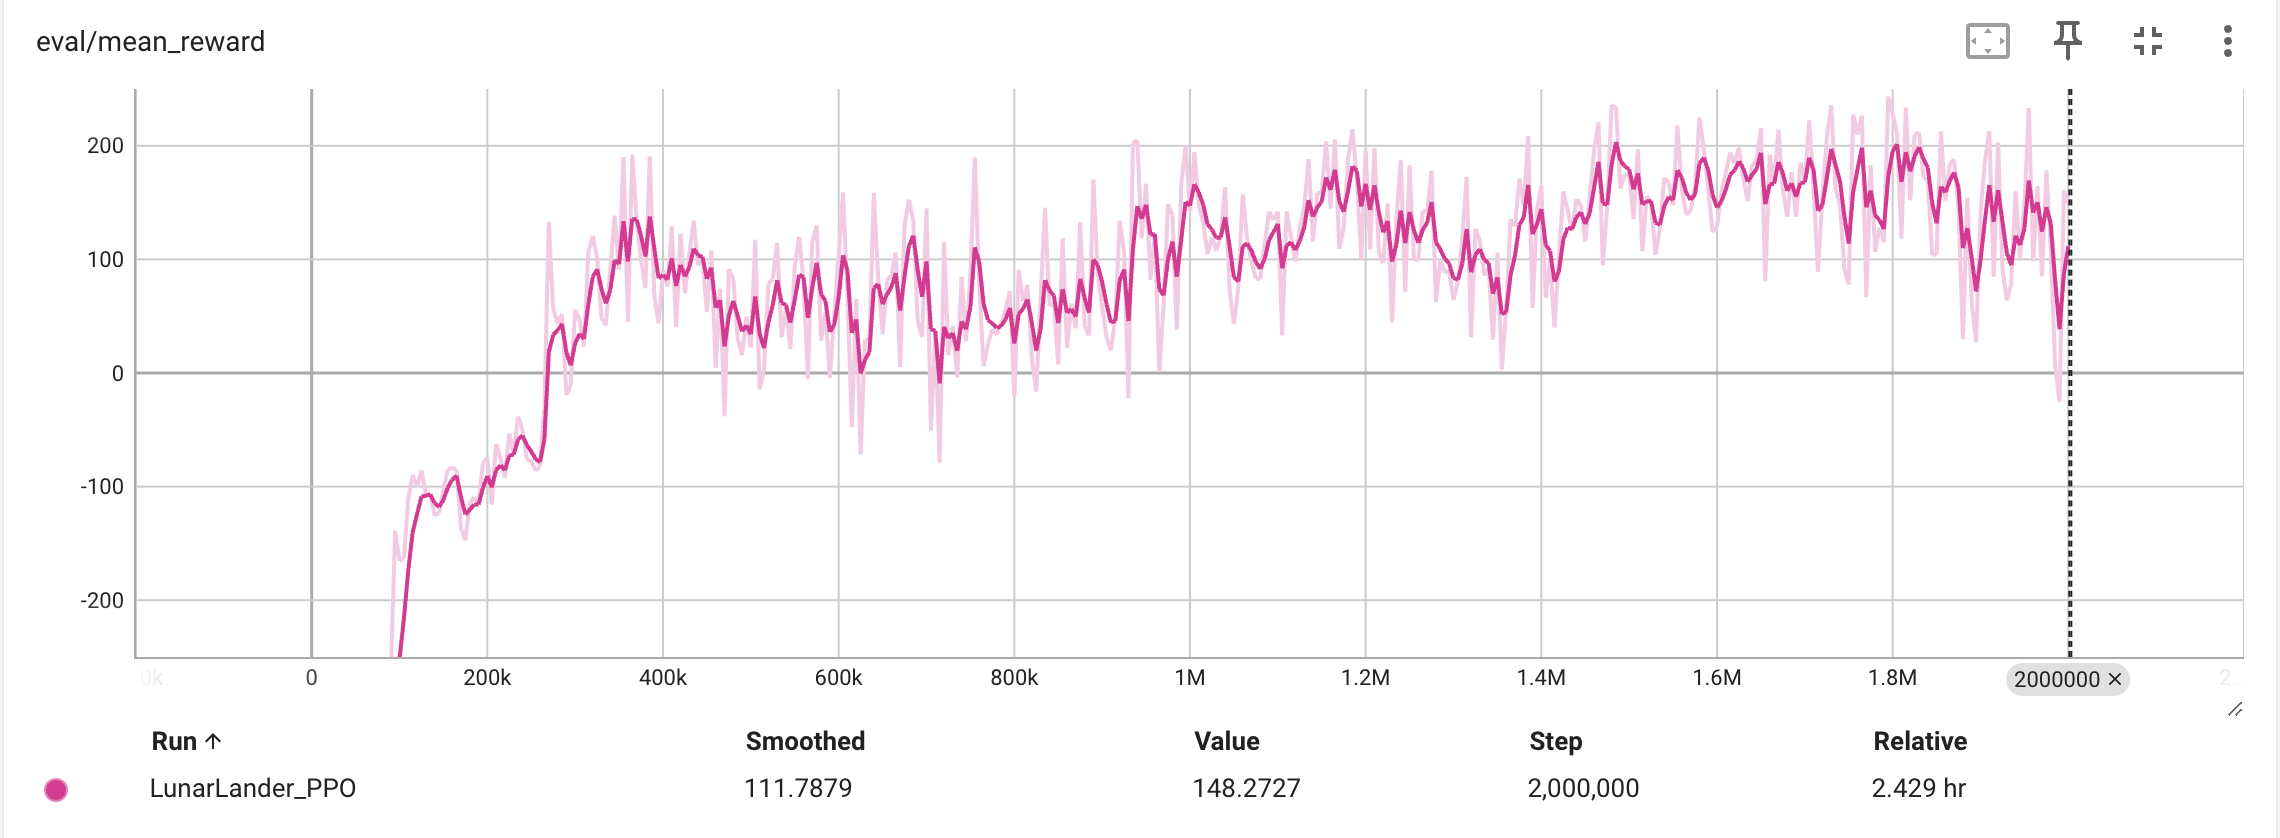
\includegraphics[width=\linewidth]{assets/4.1/LunarLander_PPO.png}
    \caption{LunarLander-v3}
  \end{subfigure}
  \vskip 0.5em
  \begin{subfigure}{0.9\linewidth}
    \centering
    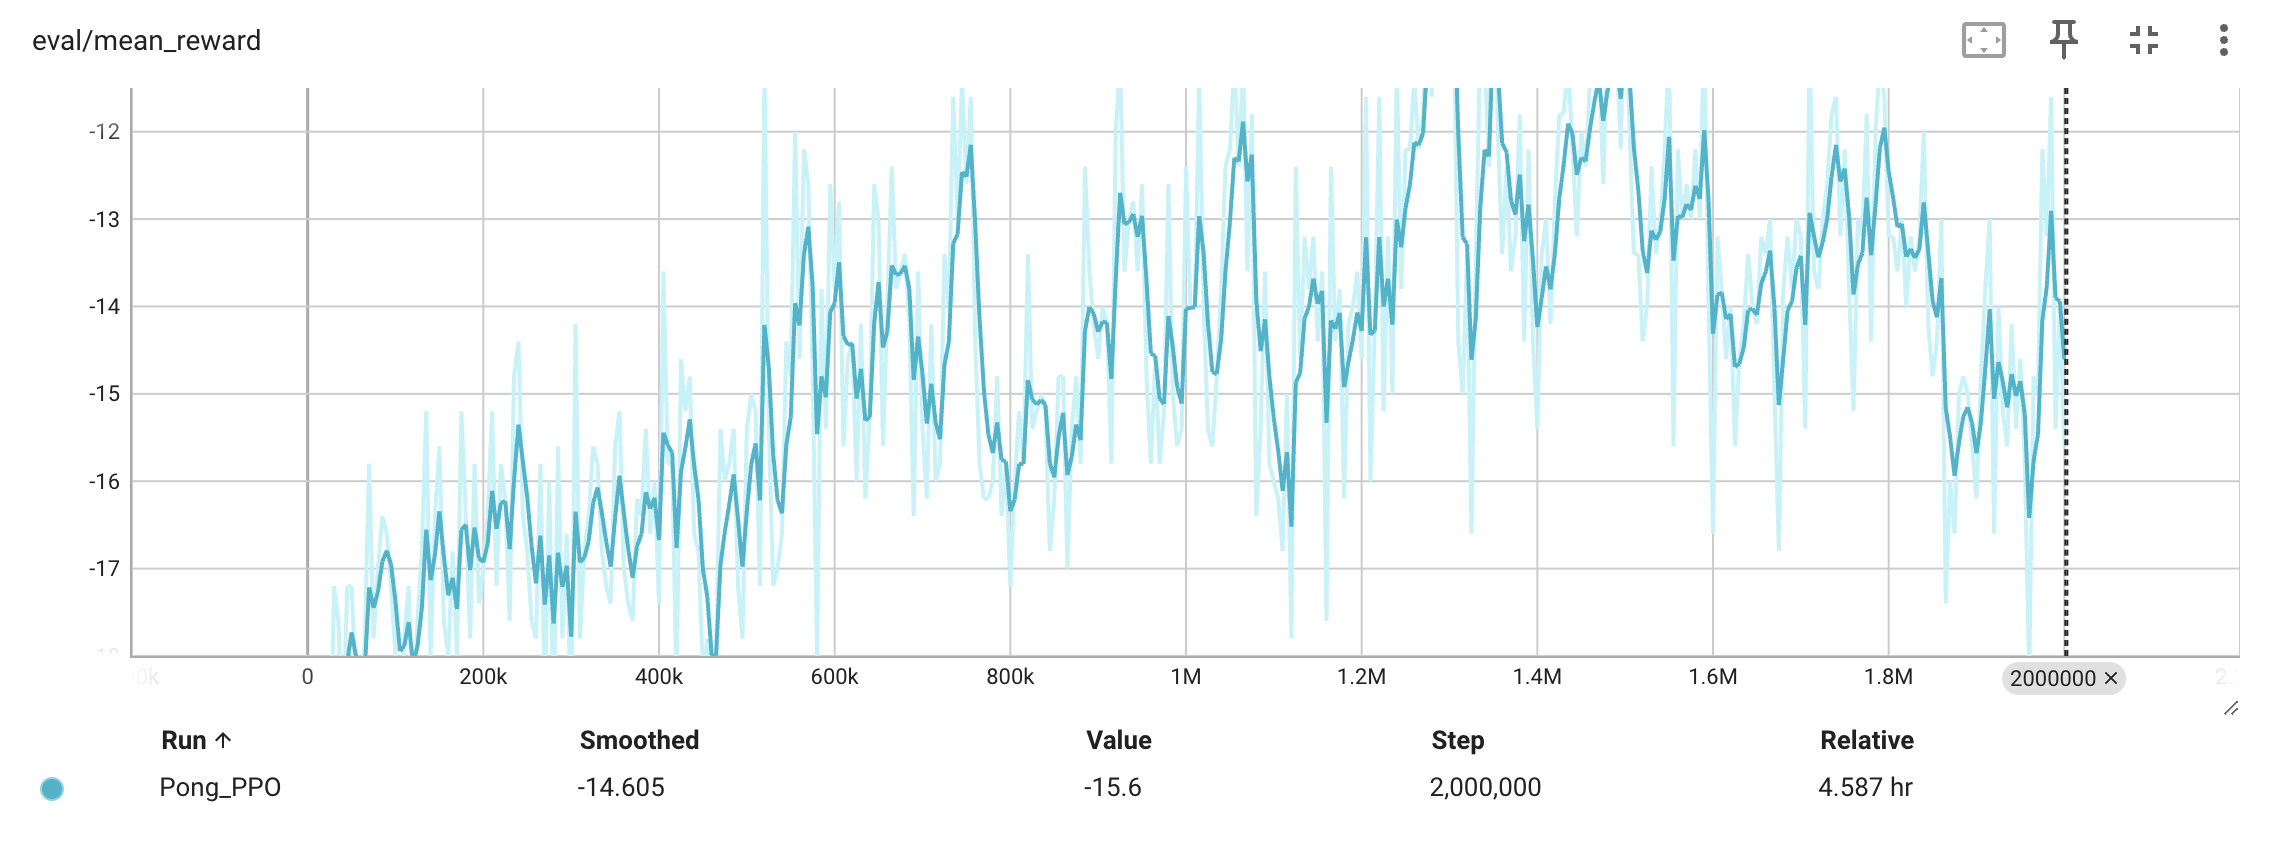
\includegraphics[width=\linewidth]{assets/4.1/Pong_PPO.png}
    \caption{Pong-v5}
  \end{subfigure}
  \caption{PPO reward curves for different environments. Each was trained for 2 million timesteps with batch size 128.}
  \label{fig:ppo_convergence}
\end{figure}


\noindent
From the reward curves, I observe the following:

\begin{itemize}
  \item \textbf{Pendulum-v1} converges rapidly and stably, reaching near-optimal performance at around 500k steps, with rewards oscillating in a narrow range.
  \item \textbf{LunarLander-v3} also converges fairly quickly around 400k steps, reaching a reward of 100. However, it exhibits higher variance and oscillation, typically between 100 and 200.
  \item \textbf{Pong-v5} shows the slowest and least stable learning progress. The reward curve exhibits large fluctuations and fails to reach high performance within 2M steps.
\end{itemize}

We hypothesize that the differences in convergence behavior stem from inherent properties of the environments (see Table~\ref{tab:env_comparison}):

\begin{itemize}
  \item \textbf{State space complexity}: Pendulum has the lowest-dimensional state (3D), LunarLander is moderate (8D), while Pong requires interpreting raw pixel images of size $210 \times 160 \times 3$.
  \item \textbf{Observation type}: Pong uses raw image input, placing heavy reliance on CNN feature extraction, while the other two environments provide structured, low-dimensional observations.
  \item \textbf{Reward sparsity}: Pong provides sparse rewards (only on point scores), which leads to more difficult credit assignment for policy updates.
  \item \textbf{Episode length}: Pong episodes last significantly longer, requiring the agent to interact over more frames before receiving reward signals, delaying learning feedback.
\end{itemize}

\subsection{Batch Size}
To investigate the effect of batch size on learning, we conducted experiments using the same algorithm (either PPO or DQN) across four batch sizes: 32, 64, 128, and 256. The experiments were repeated for three different environments: Pong-v5, LunarLander-v3, and Pendulum-v1. The results are visualized in Figure~\ref{fig:batch_comparison}.

\begin{figure}[h]
  \centering
  \begin{subfigure}{0.85\linewidth}
    \centering
    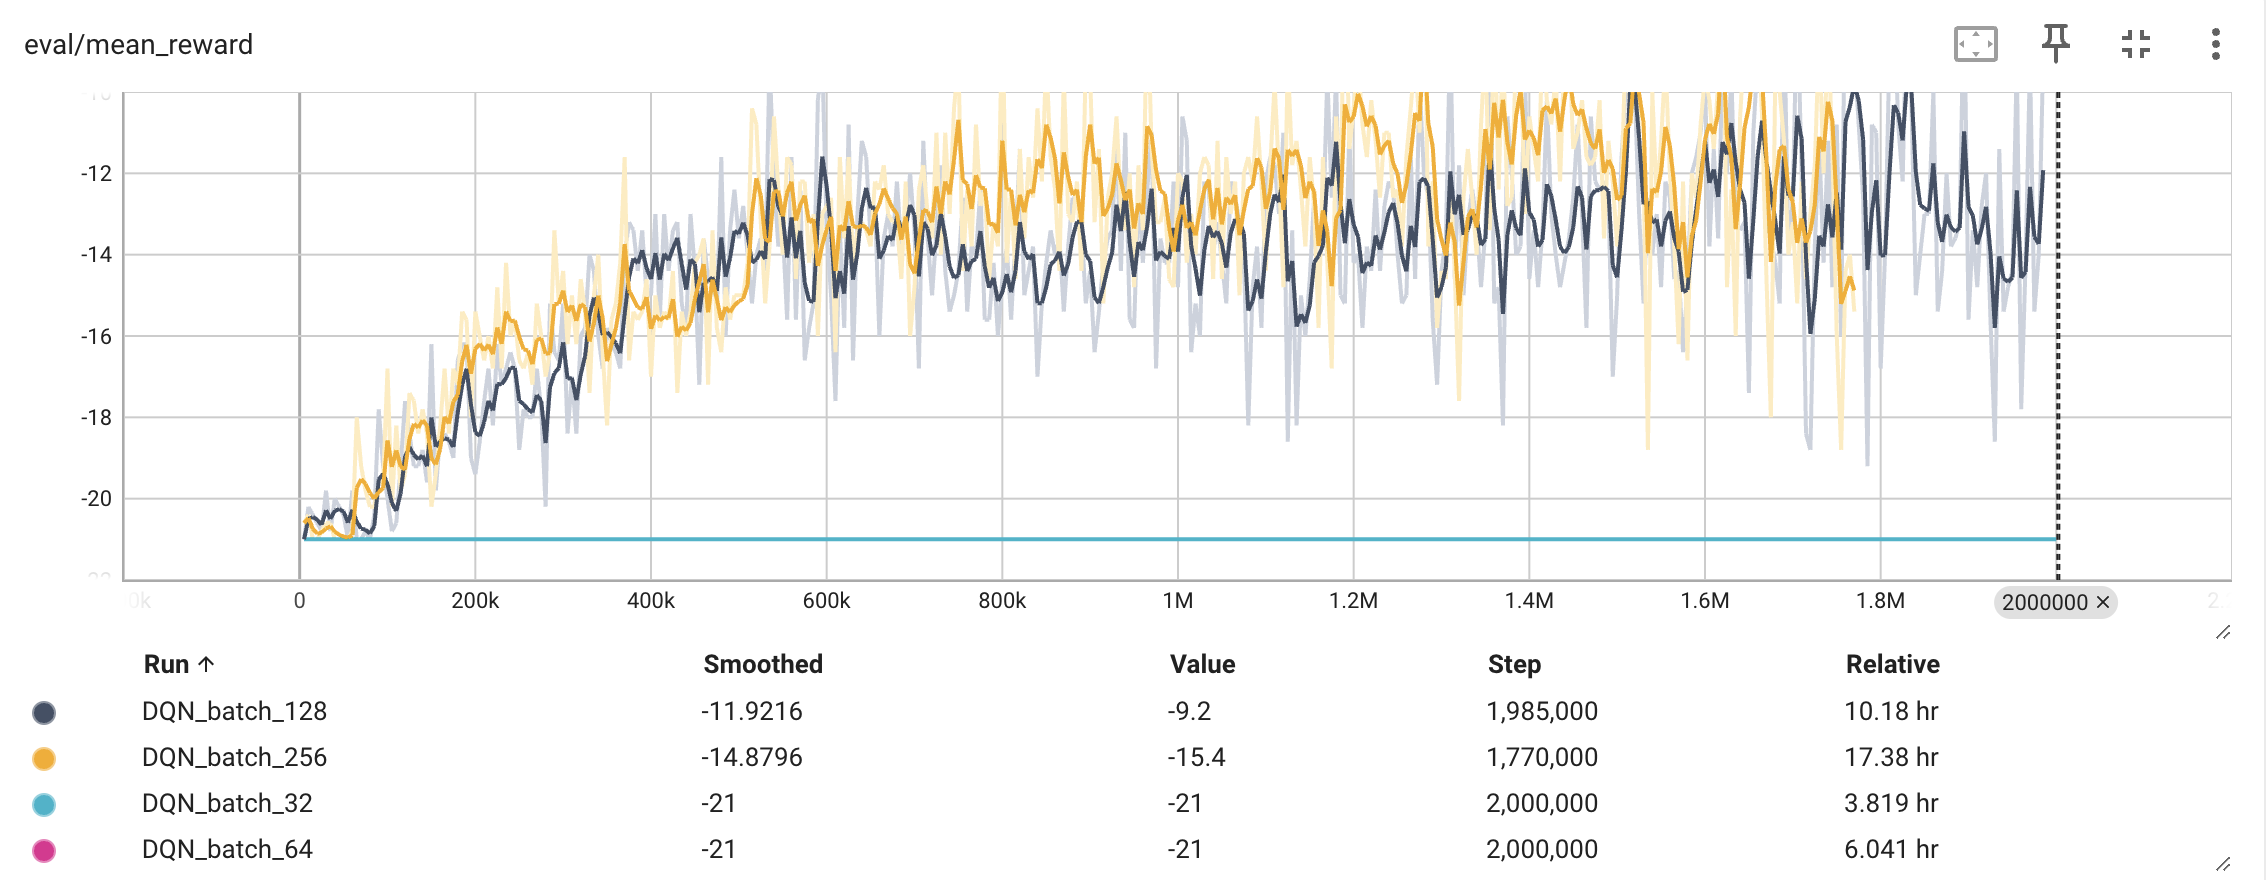
\includegraphics[width=\linewidth]{assets/4.2/Pong.png}
    \caption{DQN on Pong-v5}
  \end{subfigure}
  \vskip 0.5em
  \begin{subfigure}{0.85\linewidth}
    \centering
    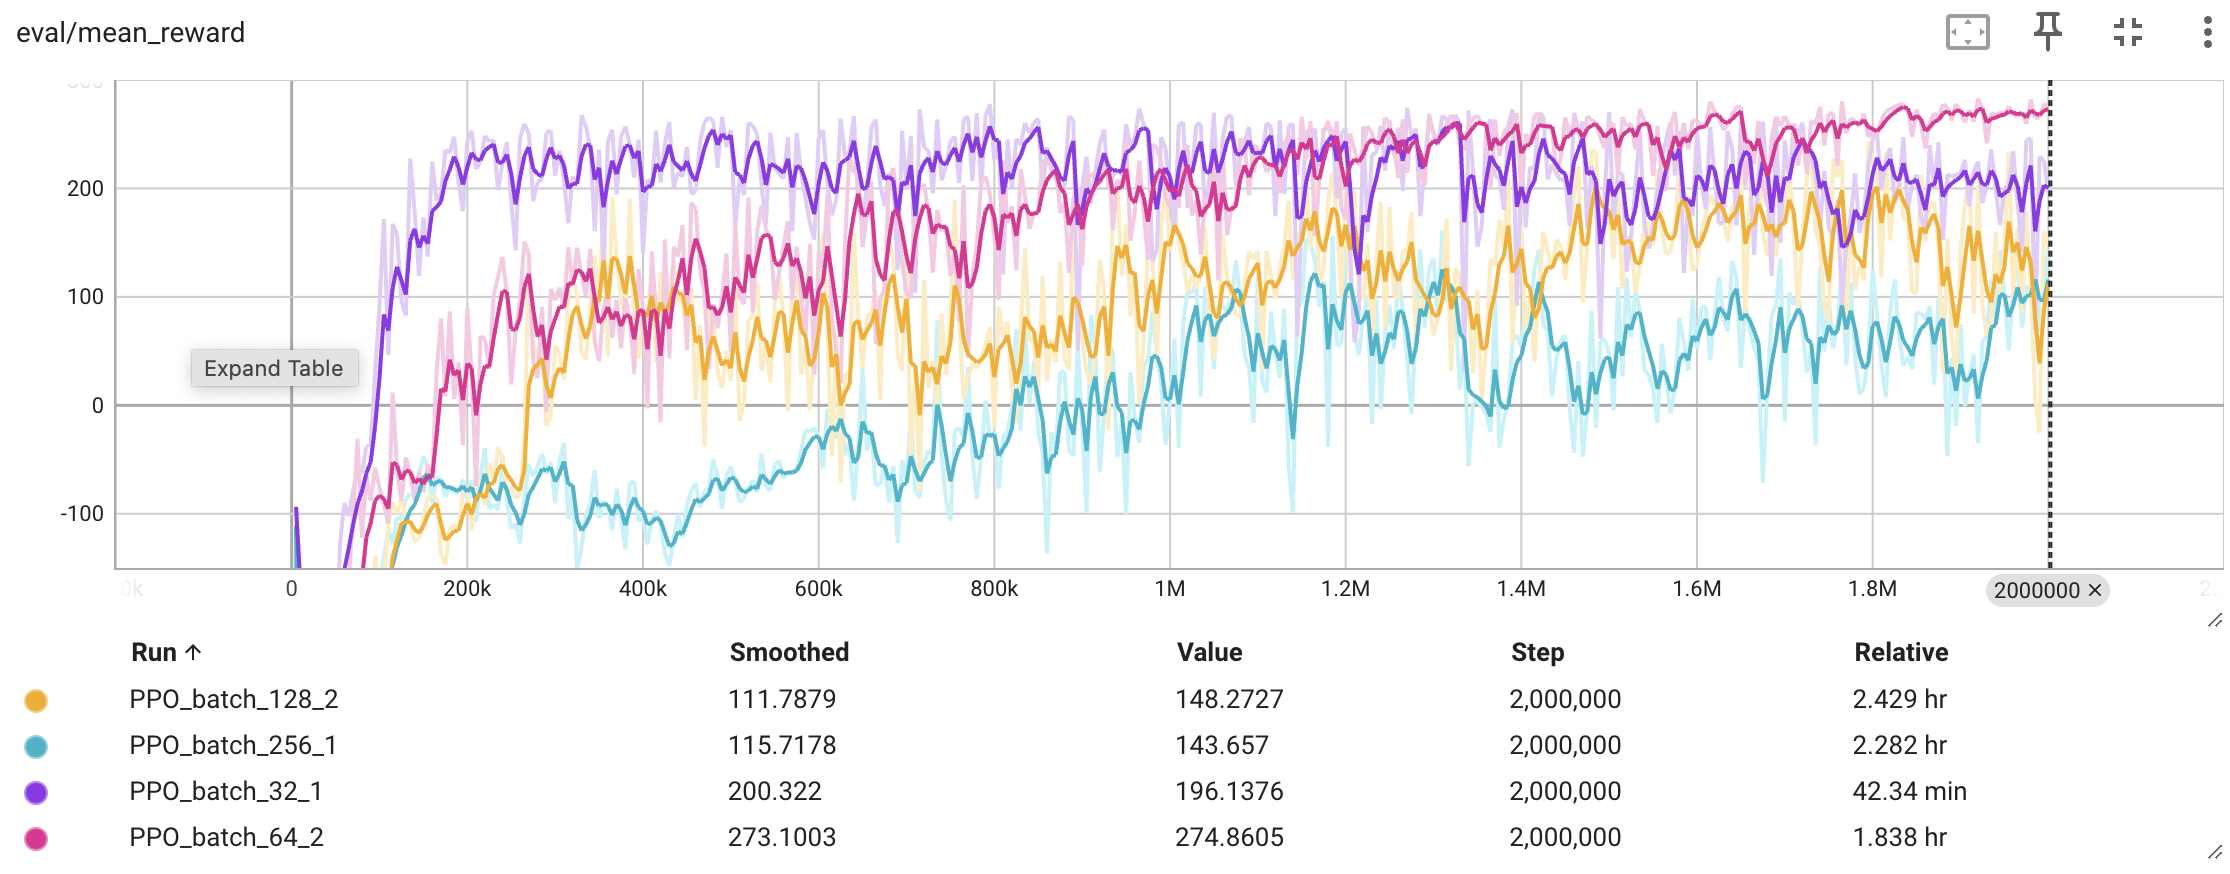
\includegraphics[width=\linewidth]{assets/4.2/LunarLander.png}
    \caption{PPO on LunarLander-v3}
  \end{subfigure}
  \vskip 0.5em
  \begin{subfigure}{0.85\linewidth}
    \centering
    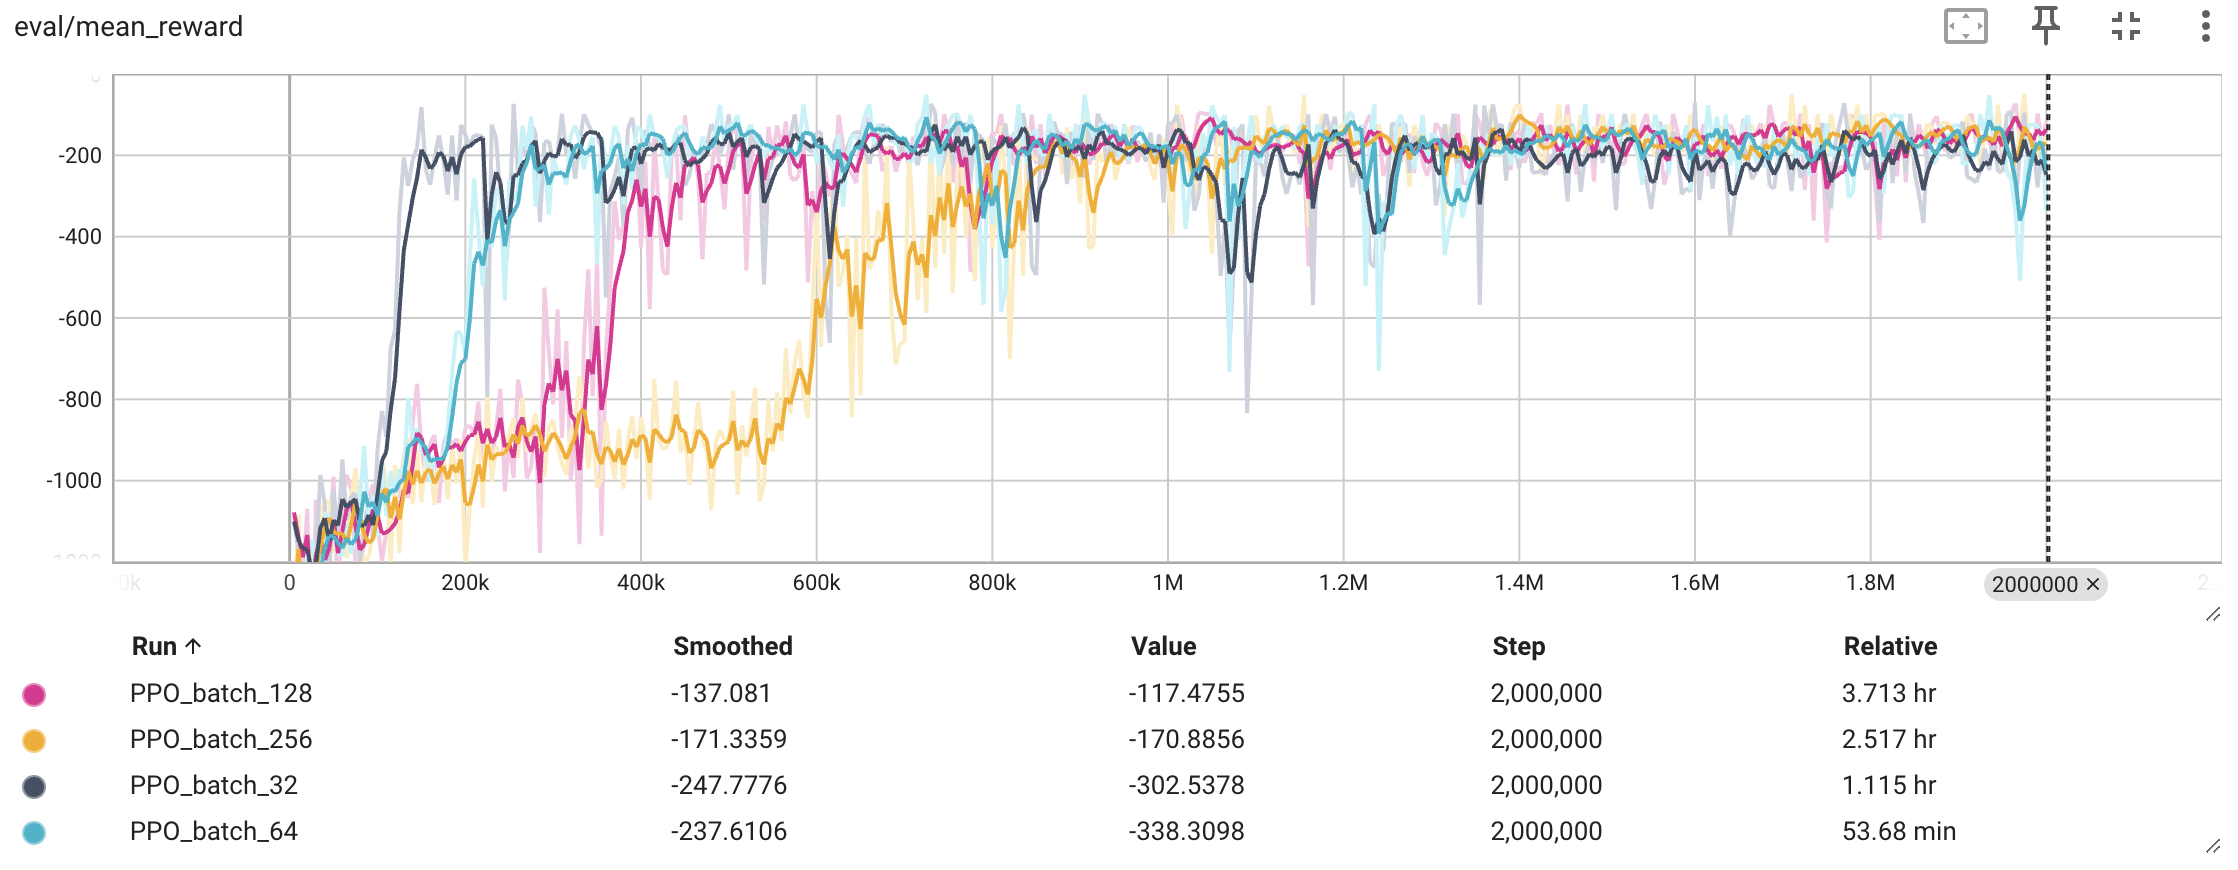
\includegraphics[width=\linewidth]{assets/4.2/Pendulum.png}
    \caption{PPO on Pendulum-v1}
  \end{subfigure}
  \caption{Effect of different batch sizes (32, 64, 128, 256) on reward convergence in three environments.}
  \label{fig:batch_comparison}
\end{figure}

\subsubsection{Pong-v5 (DQN)}
When using small batch sizes (32 or 64), the agent completely fails to learn, with the mean reward remaining flat at the minimum value of -21 throughout training. This is likely due to the sparse nature of rewards in Pong—successful experiences are rare in the early training phase. A small batch size increases the chance of drawing only uninformative transitions, making it hard for the Q-network to bootstrap meaningful updates. Batch size 128 starts to learn slowly, and 256 shows marginal improvement in stability.

\subsubsection{LunarLander-v3 (PPO)}
In contrast, smaller batch sizes (e.g., 32, 64) appear to converge to higher average rewards than larger ones in LunarLander. A plausible explanation is that smaller batches introduce more stochasticity in gradient estimation, which could act as an implicit exploration mechanism or regularization, especially in moderately shaped environments like LunarLander. Larger batch sizes may overfit to fewer high-reward strategies early on, becoming less flexible later.

\subsubsection{Pendulum-v1 (PPO)}  
I observe that smaller batch sizes lead to significantly faster convergence in Pendulum. The convergence points approximately double with each increase in batch size (around 100k, 200k, 400k, and 800k steps). One possible reason is that Pendulum has a low-dimensional, dense-reward setting, and its dynamics are relatively smooth. Small batch sizes can quickly capture enough useful gradients to adjust the policy without over-smoothing updates. In contrast, larger batches average over many redundant samples, delaying the policy shift toward the optimal region.

\subsection{Algorithms}
To compare the learning performance of different algorithms under the same setting, I ran PPO, DQN, and A2C on Pong-v5 with a fixed batch size of 128 and 2 million timesteps. The results are shown in Figure~\ref{fig:algo_comparison}.

\begin{figure}[h]
  \centering
  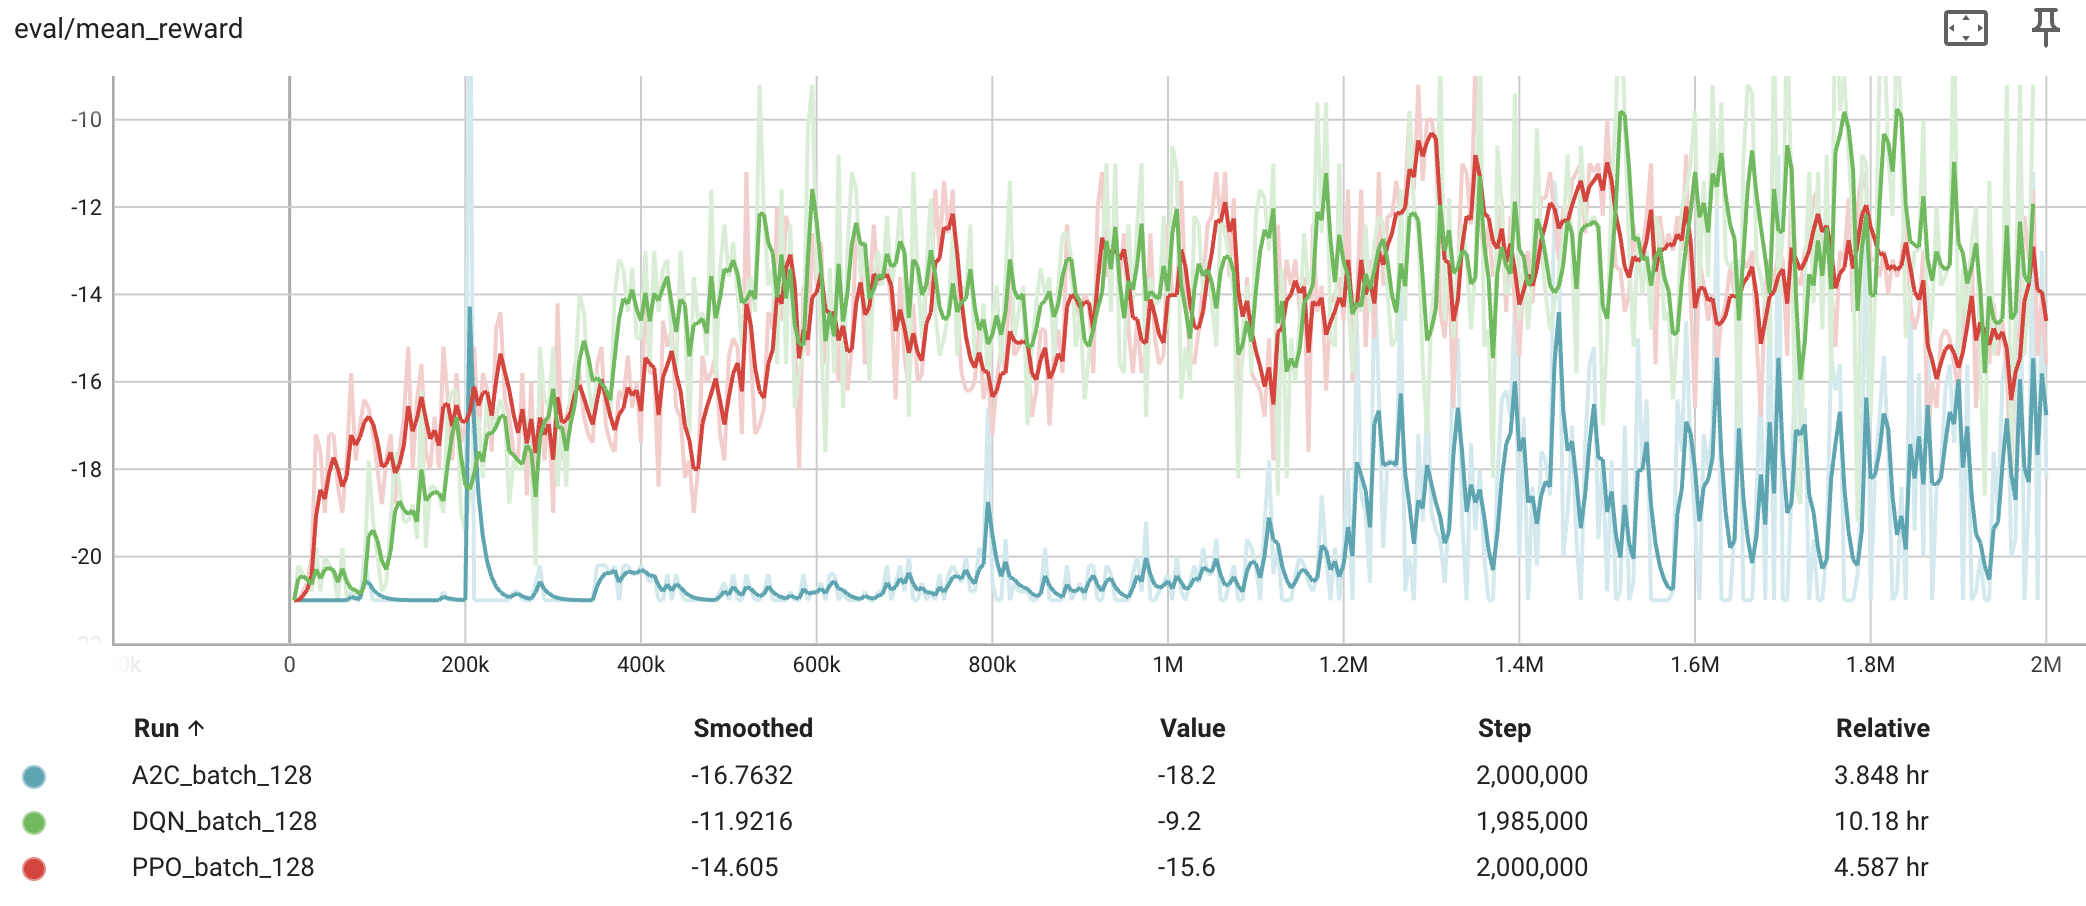
\includegraphics[width=0.95\linewidth]{assets/4.3/Pong_algorithms.png}
  \caption{Mean episode reward of PPO, DQN, and A2C on Pong-v5 with batch size 128.}
  \label{fig:algo_comparison}
\end{figure}

\noindent
From the reward curves, we observe the following:

\begin{itemize}
  \item \textbf{PPO and DQN} both demonstrate gradual learning, with DQN achieving slightly higher final rewards than PPO. However, the difference in performance is not significant.
  \item \textbf{Training time}, on the other hand, shows a clear gap. DQN took more than twice the training time compared to PPO to reach similar performance. This is likely due to the extra cost from the experience replay buffer and frequent Q-network updates.
  \item \textbf{A2C} underperforms significantly. While it shows some learning trend, the average reward remains close to the minimum for most of the training period, with high variance and no stable improvement. This suggests that A2C struggles in environments with sparse rewards like Pong, especially without extra tricks like entropy tuning or parallel environments.
\end{itemize}

\noindent
These results indicate that for sparse-reward environments like Pong, value-based methods (DQN) and policy-based methods (PPO) can both be effective, but PPO may be more practical due to its faster training. A2C, while efficient in shaped-reward environments, is less suitable for Atari-style games without significant modification.

\subsection{DQN Experiments}

\subsubsection{Hard Update vs. Soft Update}
In Stable-Baselines3, DQN uses a hard update strategy by default, where the target network is updated every fixed number of steps. To evaluate the impact of soft updates, we modified the update method using the parameter \texttt{tau}, which controls the Polyak averaging factor (See Table~\ref{tab:dqn_update}).

\begin{table}
  \centering
  \begin{tabular}{@{}l>{\centering\arraybackslash}p{1.5cm} >{\raggedright\arraybackslash}p{4.2cm}@{}}
    \toprule
    Configuration & $\tau$ & Target network update \\
    \midrule
    \textbf{Hard update} & 1.0 & Copied from the main network every fixed interval. \\
    \textbf{Soft update} & 0.005 & Updated slowly using Polyak averaging: $\theta_{\text{target}} \leftarrow \tau \theta + (1 - \tau)\theta_{\text{target}}$. \\
    \bottomrule
  \end{tabular}
  \caption{Comparison of DQN update strategies on Pong.}
  \label{tab:dqn_update}
\end{table}

We set \texttt{tau = 0.005} to enable soft updates while keeping the batch size at 128. As shown in Figure~\ref{fig:dqn_update}, the learning performance deteriorates significantly under soft update—the agent fails to learn a meaningful policy and reward remains flat near the minimum.

\begin{figure}[h]
  \centering
  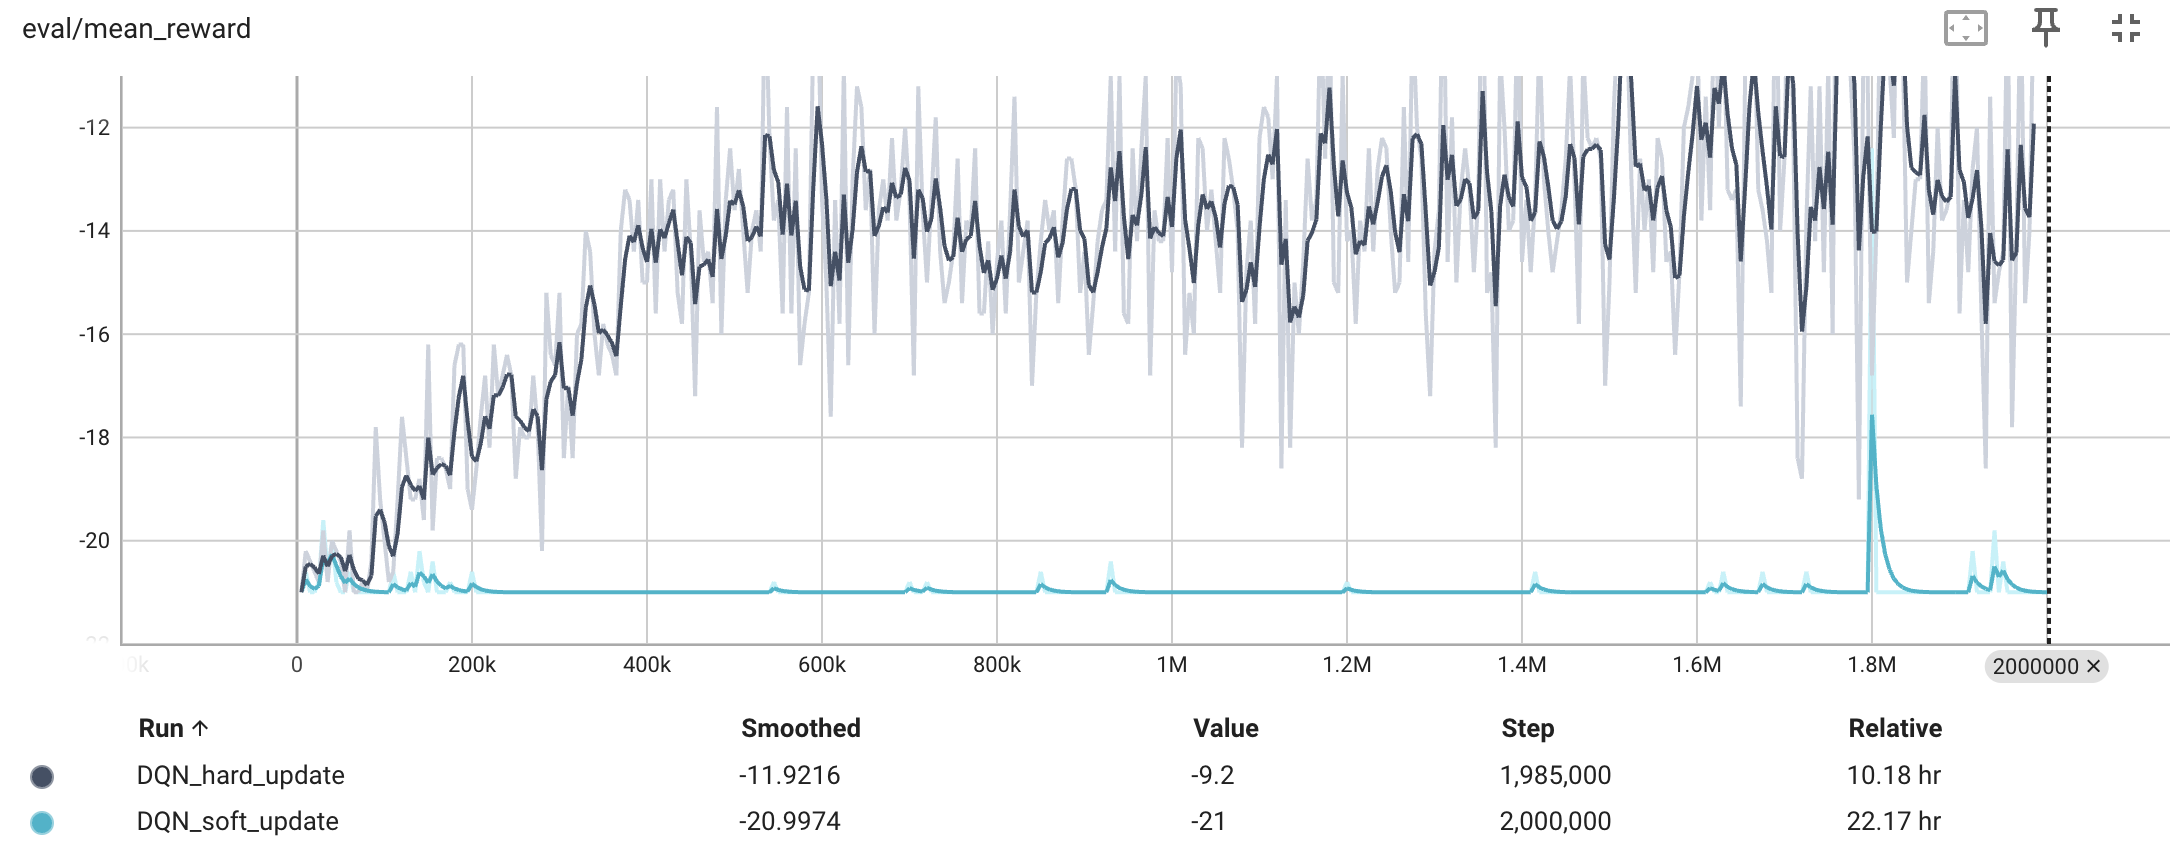
\includegraphics[width=0.95\linewidth]{assets/4.4/Hard_vs_Soft.png}
  \caption{Performance comparison of DQN with hard update (default) and soft update ($\tau=0.005$).}
  \label{fig:dqn_update}
\end{figure}

This result suggests that for environments like Pong with sparse rewards, target stability is important, and soft updates may be too conservative to enable efficient Q-value propagation.

\subsubsection{Exploration vs. Exploitation Tradeoff}

\begin{table}
  \centering
  \begin{tabular}{@{}lcc>{\raggedright\arraybackslash}p{4.1cm}@{}}
    \toprule
    Group & Final $\epsilon$ & Fraction & Notes \\
    \midrule
    \textbf{A} & 0.05 & 0.1 & Fastest convergence; favors early exploitation. \\
    \textbf{B} & 0.01 & 0.5 & Longer exploration phase. \\
    \textbf{C} & 0.10 & 0.3 & Balanced between exploration and exploitation. \\
    \bottomrule
  \end{tabular}
  \caption{Comparison of $\epsilon$-greedy decay schedules in DQN on Pong.}
  \label{tab:dqn_exploration}
\end{table}


To analyze the effect of $\epsilon$-greedy decay scheduling, we tested three groups of exploration settings with the same initial $\epsilon=1.0$ but different final values and decay fractions (see Table~\ref{tab:dqn_exploration}).

\begin{figure}[h]
  \centering
  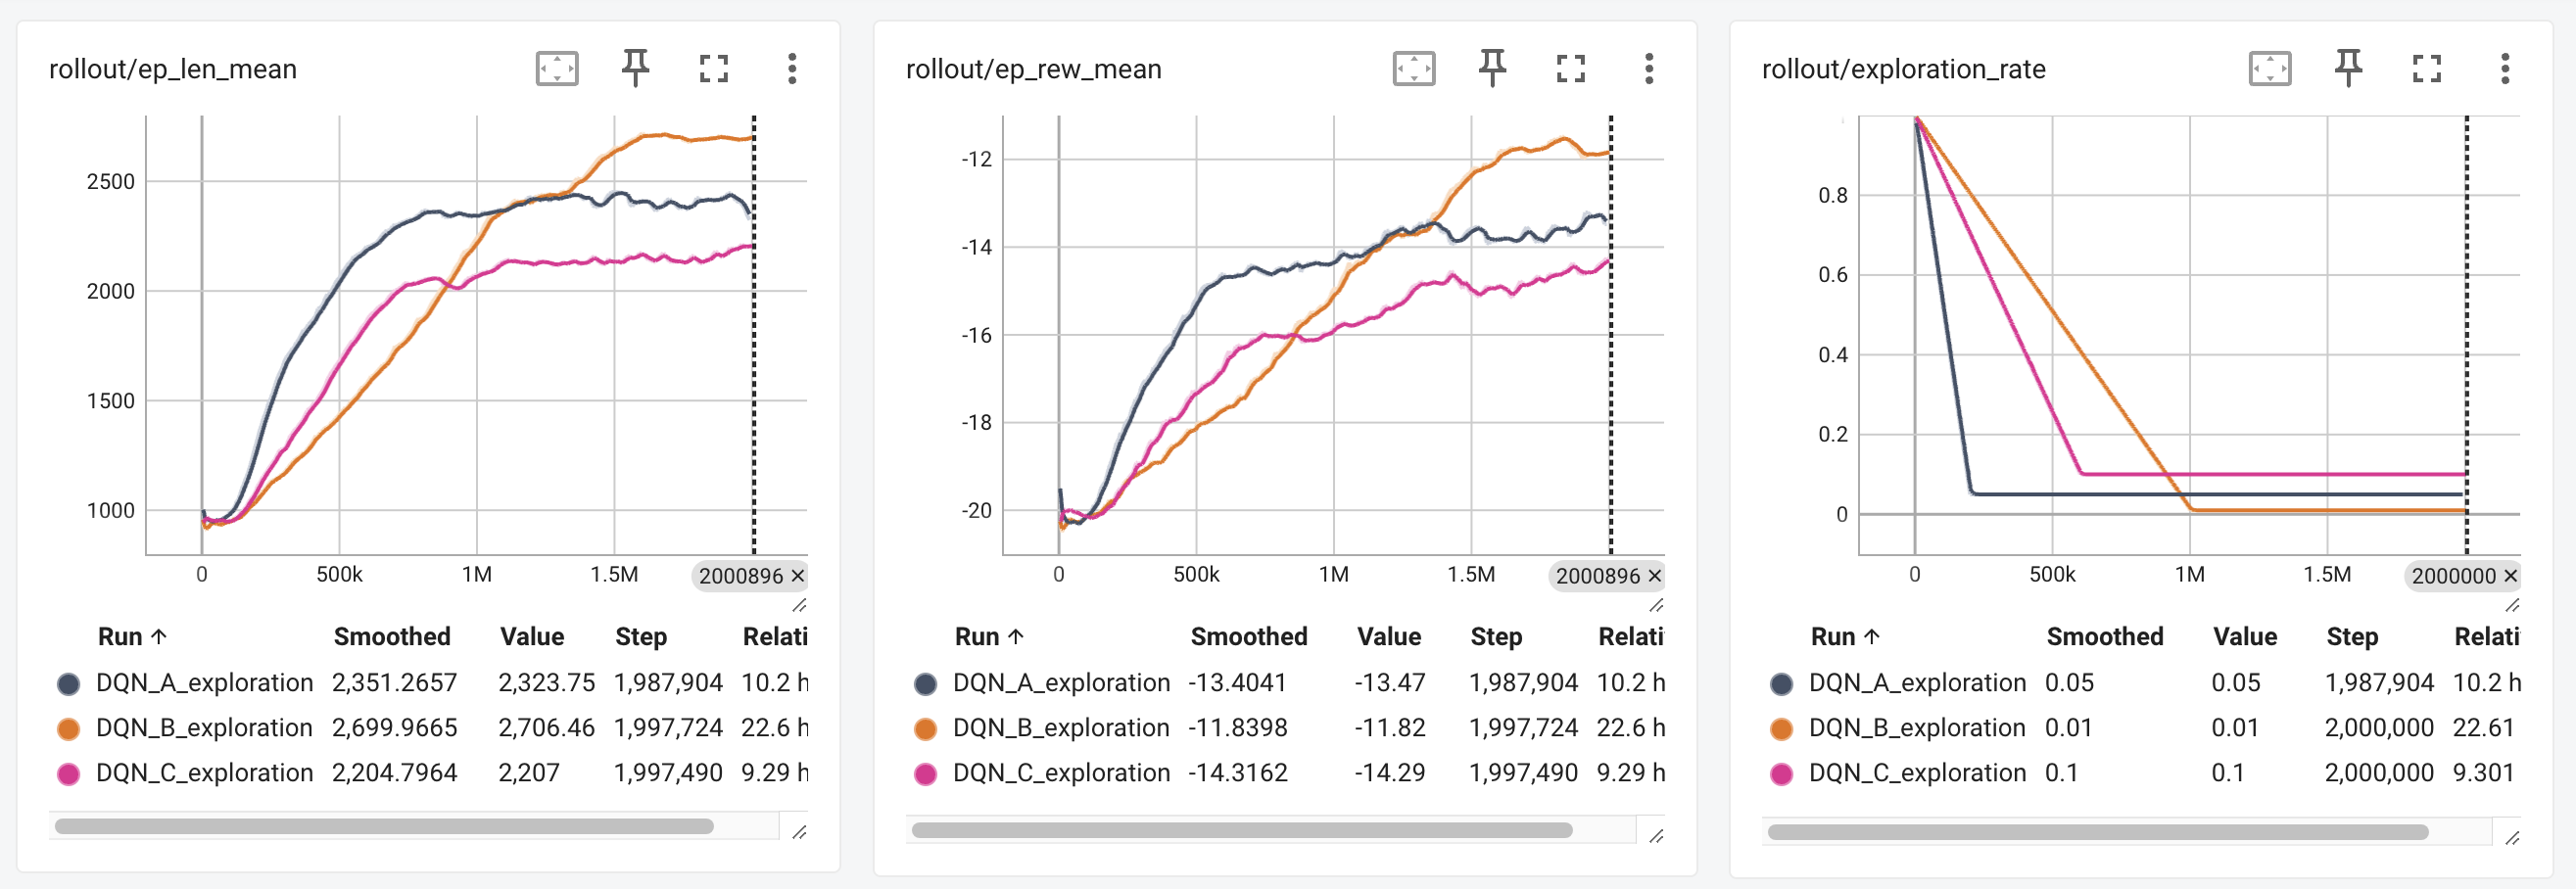
\includegraphics[width=\linewidth]{assets/4.4/Epsilon_Comparison.png}
  \caption{Reward, episode length, and exploration rate for different $\epsilon$-decay schedules.}
  \label{fig:epsilon_result}
\end{figure}

\noindent
From the experimental results (see Figure~\ref{fig:epsilon_result}), we observe the following:

\begin{itemize}
  \item \textbf{Group A} converges the fastest and shows stable learning behavior early on, but plateaus at a slightly lower reward ($\sim -13.4$). The early exploitation allows quick policy refinement but may lead to local optima due to insufficient exploration.
  
  \item \textbf{Group B} achieves the highest final reward ($\sim -11.8$), though its learning process is initially slower. The prolonged exploration phase helps gather a diverse set of transitions, allowing the Q-network to generalize better and avoid premature convergence.
  
  \item \textbf{Group C} underperforms in both reward and learning speed. Its final reward is the lowest ($\sim -14.3$), and its episode length stabilizes at a lower level. The decay schedule might be too shallow to encourage deep exploration, but not aggressive enough to exploit effectively.
\end{itemize}

We conclude that in sparse-reward environments like Pong, a longer exploration phase (as in Group B) may lead to better long-term performance, despite a slower start. Fast decay (Group A) can offer quicker results but risks suboptimal convergence. Balanced decay (Group C) might fail to provide a strong signal in either direction, resulting in mediocre performance.



%------------------------------------------------------------------------
\section{Discussion}
\label{sec:discussion}

\subsection{RL Algorithm and Environment Specificity}

Through the experiments, it became evident that no single RL algorithm or configuration universally performs best across all environments. For instance, PPO works exceptionally well in low-dimensional, dense-reward settings like Pendulum, but struggles in sparse-reward tasks like Pong without proper tuning. DQN performs better in Pong but requires more training time and is sensitive to batch size and $\epsilon$ decay scheduling. This highlights the importance of adapting algorithm choices and hyperparameters based on the characteristics of the environment—state representation, reward density, and episode dynamics all play a crucial role.

\subsection{Using CPU or GPU?}

Contrary to initial expectations, using a GPU does not always result in faster training. For lightweight models such as \texttt{MlpPolicy} applied to environments like Pendulum or LunarLander, CPU execution can be more efficient. This is because the overhead of transferring data between CPU and GPU can exceed the speedup gained from parallelization, especially when the model is small or the batch size is limited. On the other hand, environments with image inputs (e.g., Pong) and policies like \texttt{CnnPolicy} benefit significantly from GPU acceleration.

\subsection{Lessons Learned}

This project provided a deeper understanding of the nuances in training reinforcement learning agents. The experiments showed that:
\begin{itemize}
  \item Sparse rewards are particularly challenging for value-based methods, and careful tuning of exploration strategies is crucial.
  \item Hyperparameters such as batch size, update frequency, and exploration schedules have dramatic effects on convergence speed and final performance.
  \item Empirical experimentation is indispensable—many insights (e.g., GPU being slower in small models) would not be obvious without hands-on trials.
\end{itemize}

Overall, the experience reinforced the idea that reinforcement learning is highly context-sensitive, and success depends not just on choosing a good algorithm, but on tailoring it to the environment’s properties and the computational setup.

%%%%%%%%% REFERENCES
{\small
\bibliographystyle{ieee_fullname}
\bibliography{egbib}
}

\end{document}
